% !TEX root = main.tex
\chapter[head={The CKM angle $\gamma$},tocentry={The CKM angle $\symbfsf{\gamma}$}]{The CKM angle $\symbfsf{\gamma}$}
\label{ch:CKMAngleGamma}

The unitarity of the CKM matrix yields to several constraints which can be presented as triangles in the complex plane.
Overconstraining these triangles give a nice self consistency check of the theory of the \ac{SM}.
The CKM angle $\gamma$ is one angle in the triangle introduced in \cref{eq:CKMtriangle}.
In \cref{fig:ckmtriangle} the current experimental cosntraints on the triangle are shown.
It can be seen that $\gamma$ is the least well know parameter of the triangle to date.
This chapter is organised as follows: Firstly it is described how the angle $\gamma$ can be accessed in section \cref{sec:accessGamma} and how it can be measured in decays of charged \B mesons (\cref{sec:gammainChargedModes}).
Then the effect of \CP violation in the decay mode \BdToDpi is described in \cref{sec:cpvInBd2Dpi} and how this gives a handle on the angle $\gamma$ (\cref{sec:GammaInBd2Dpi}).

\begin{figure}[tbp]
	\centering
	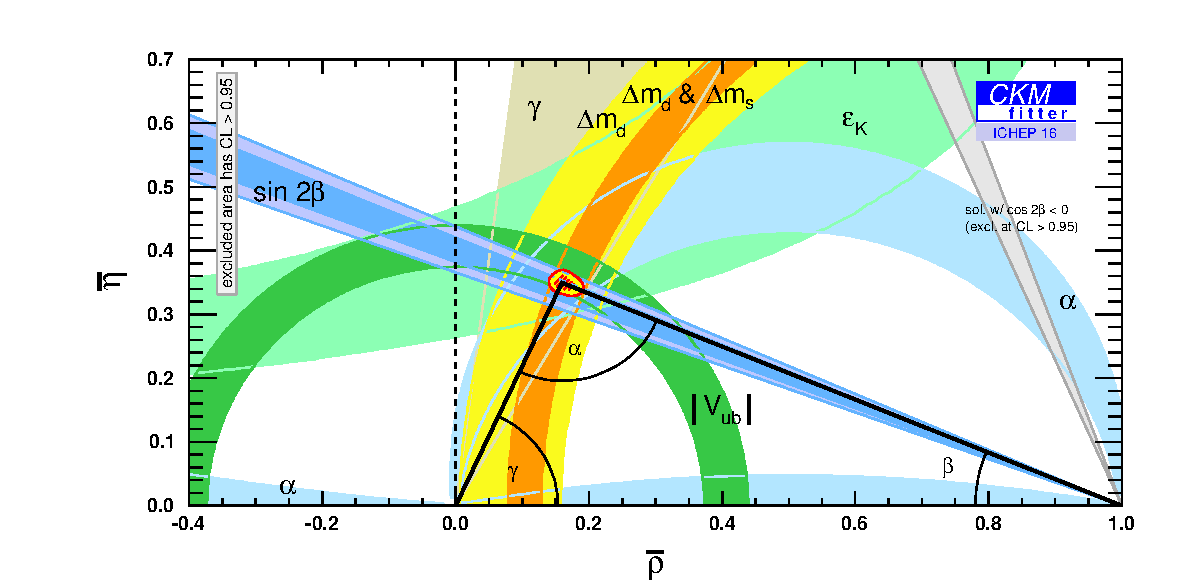
\includegraphics[width=0.8\textwidth]{04gamma/figs/CKMTriangle.pdf}
	\caption{CKM triangle in the complex plane.
	The coloured bands show the experimental constraints.
	The red hashed and the yellow area around the apex represents the currrent ucnertainties at \SI{68}{\percent} and \SI{95}{\percent} confidence level, respectively~\cite{CKMfitter2005}.}
	\label{fig:ckmtriangle}
\end{figure}

\section[head={Accessing the angle $\gamma$},tocentry={Accessing the angle $\gamma$}]{Accessing the angle $\symbfsf{\gamma}$}
\label{sec:accessGamma}

The angle $\gamma$ can be determined by exploiting the interference between favoured transitions $\bquark\to\cquark$ and suppressed transitions $\bquark\to\uquark$.
Hence it can be determined by just measuring tree-level decays.
However as $\gamma$ is the phase of the matrix element \Vub, decays in which it can be measured are highly suppressed and often suffer a non-negligible pollution from transitions containing loops.


\section[head={Measuring the angle $\gamma$ in charged \B decays},tocentry={Measuring the angle $\gamma$ in charged \B decays}]{Measuring the angle $\symbfsf{\gamma}$ in charged $\symbfsf{\B}$ decays}
\label{sec:gammainChargedModes}

\Blindtext

\section[head={\CP violation in $\Bz\to\Dm\pip$},tocentry={\CP violation in $\Bz\to\Dm\pip$}]{$\symbfsf{\CP}$ violation in $\symbfsf{\Bz\to\Dm\pip}$}
\label{sec:cpvInBd2Dpi}

Using then the time evolution presented in \cref{sec:TimeEvolution} the probability for the transitions $\left|\left<\,f\,\Big|T\Big|\Bz\!(t)\right>\right|^2$ can be calculated.
Here $\Bz\!(t)$ ($\Bzb\!(t)$) denotes a \B meson which was produced as a \Bz (\Bzb) at $t=0$:
\begin{align}
\left|\left<\,\f\,\Big|T\Big|\Bz\!(t)\right>\right|^2 =&
\left|\left<\,\f\,\Big|T\Big|\Bz\right>g_+-\frac{q}{p}\left<\,\f\,\Big|T\Big|\Bzb\right>g_-\right|^2\nonumber\\
=&\Af^2\left|g_+ - \frac{q}{p}\frac{\Abarf}{\Af} g_-\right|^2=\Af\left|g_+ -\Lf\,g_-\right|^2\nonumber\\
=&\Af^2\left(g_+g_+^*+\left|\Lf\right|^2g_-g_-^*-\left(\lambda_{f}^*g_-^*g_+ + \Lf\,g_+^* g_-\right)\right)
\end{align}
In analogy the probabilites for an initially produced \Bzb and a second finalstate \fbar are defined as
\begin{align}
\left|\left<\,\f\,\Big|T\Big|\Bzb\!(t)\right>\right|^2 &=
\Af^2\left|\frac{p}{q}\right|^2\left(g_+g_+^*\left|\Lf\right|^2+g_-g_-^*-\left(\Lfst g_+^*g_- + \Lf\,g_-^* g_+\right)\right)\\
\left|\left<\,\fbar\,\Big|T\Big|\Bz\!(t)\right>\right|^2 &=
\Abarfbar^2\left|\frac{q}{p}\right|^2\left(g_+g_+^*\left|\Lfbar\right|^2+g_-g_-^*-\left(\Lfbarst g_+^*g_- + \Lfbarst\,g_-^* g_+\right)\right)\\
\left|\left<\,\fbar\,\Big|T\Big|\Bzb\!(t)\right>\right|^2 &=
\Abarfbar^2\hphantom{\left|\frac{q}{p}\right|^2}\left(g_+g_+^*+\left|\Lfbar\right|^2g_-g_-^*-\left(\Lfbarst g_-^*g_+ + \Lfbar\,g_+^* g_-\right)\right)
\end{align}
Using
\begin{align}
g_{\pm}g_{\pm}^{*} &= \frac{1}{2}e^{-\Gamma t}\left(\cosh\left(\frac{\DG}{2}t\right)\pm\cos\left(\dm t\right)\right)\\
g_{\pm}^*g_{\mp} &=  \frac{1}{2}e^{-\Gamma t}\left(\sinh\left(\frac{\DG}{2}t\right)\mp i\sin\left(\dm t\right)\right)
\end{align}
the probabilities can be expressed as
\begin{align}
\left|\left<\,\f\,\Big|T\Big|\Bz\!(t)\right>\right|^2 =&
\frac{1}{2}e^{\Gamma t}\left|\Af\right|^2\left(1+\left|\Lf\right|^2\right)\hphantom{\left|\frac{p}{q}\right|^2}
\Bigg[\cosh\left(\frac{\DG}{2}t\right) + A_f^{\DG}\sinh\left(\frac{\DG}{2}t\right)\nonumber\\
&\hphantom{\frac{1}{2}e^{\Gamma t}\left|\Af\right|^2\left(1+\left|\Lf\right|^2\right)\left|\frac{p}{q}\right|^2\Bigg[}
-\Sf\sin\left(\dm t\right)+\Cf\cos\left(\dm t\right)\Bigg]\\
\left|\left<\,\f\,\Big|T\Big|\Bzb\!(t)\right>\right|^2 =&
\frac{1}{2}e^{\Gamma t}\left|\Af\right|^2\left(1+\left|\Lf\right|^2\right)\left|\frac{p}{q}\right|^2
\Bigg[\cosh\left(\frac{\DG}{2}t\right) + A_f^{\DG}\sinh\left(\frac{\DG}{2}t\right)\nonumber\\
&\hphantom{\frac{1}{2}e^{\Gamma t}\left|\Af\right|^2\left(1+\left|\Lf\right|^2\right)\left|\frac{p}{q}\right|^2\Bigg[}
+\Sf\sin\left(\dm t\right)-\Cf\cos\left(\dm t\right)\Bigg]\\
\left|\left<\,\fbar\,\Big|T\Big|\Bz\!(t)\right>\right|^2 =&
\frac{1}{2}e^{\Gamma t}\left|\Abarfbar\right|^2\left(1+\left|\Lfbar\right|^2\right)\left|\frac{q}{p}\right|^2
\Bigg[\cosh\left(\frac{\DG}{2}t\right) + A_{\kern 1.5pt\overline{\kern -1.5pt f\kern 1.5pt}}^{\DG}\sinh\left(\frac{\DG}{2}t\right)\nonumber\\
&\hphantom{\frac{1}{2}e^{\Gamma t}\left|\Af\right|^2\left(1+\left|\Lf\right|^2\right)\left|\frac{q}{p}\right|^2\Bigg[}
-\Sfbar\sin\left(\dm t\right)+\Cfbar\cos\left(\dm t\right)\Bigg]\\
\left|\left<\,\fbar\,\Big|T\Big|\Bzb\!(t)\right>\right|^2 =&
\frac{1}{2}e^{\Gamma t}\left|\Abarfbar\right|^2\left(1+\left|\Lfbar\right|^2\right)\hphantom{\left|\frac{q}{p}\right|^2}
\Bigg[\cosh\left(\frac{\DG}{2}t\right) + A_{\kern 1.5pt\overline{\kern -1.5pt f\kern 1.5pt}}^{\DG}\sinh\left(\frac{\DG}{2}t\right)\nonumber\\
&\hphantom{\frac{1}{2}e^{\Gamma t}\left|\Af\right|^2\left(1+\left|\Lf\right|^2\right)\left|\frac{q}{p}\right|^2\Bigg[}
+\Sfbar\sin\left(\dm t\right)-\Cfbar\cos\left(\dm t\right)\Bigg]
\end{align}
with the \CP coefficients
\begin{align}
A_f^{\DG}&=-\frac{2\mathcal{Re}\left(\Lf\right)}{1+\left|\Lf\right|^2}\hspace{0.5cm}
\Sf=\frac{2\mathcal{Im}\left(\Lf\right)}{1+\left|\Lf\right|^2}\hspace{0.5cm}
\Cf=\frac{1-\left|\Lf\right|^2}{1+\left|\Lf\right|^2}\\
A_{\kern 1.5pt\overline{\kern -1.5pt f\kern 1.5pt}}^{\DG}&=-\frac{2\mathcal{Re}\left(\Lfbar\right)}{1+\left|\Lfbar\right|^2}\hspace{0.5cm}
\Sfbar=-\frac{2\mathcal{Im}\left(\Lfbar\right)}{1+\left|\Lfbar\right|^2}\hspace{0.5cm}
\Cfbar=-\frac{1-\left|\Lfbar\right|^2}{1+\left|\Lfbar\right|^2}.
\end{align}
\begin{equation}
\vspace{3cm}
\end{equation}
Considering now the case where direct and indirect \CP violation are neglibile ($\left|\Lf\right|=\pm1$ and $\left|\Lfbar\right|=\pm1$) the asymmetries
\begin{align}
\frac{\left|\left<\,\f\,\Big|T\Big|\Bz\!(t)\right>\right|^2 - \left|\left<\,\f\,\Big|T\Big|\Bzb\!(t)\right>\right|^2}{\left|\left<\,\f\,\Big|T\Big|\Bz\!(t)\right>\right|^2 + \left|\left<\,\f\,\Big|T\Big|\Bzb\!(t)\right>\right|^2}
= \frac{\Cf\cos\left(\dm t\right) - \Sf\sin\left(\dm t\right)}{\cosh\left(\frac{\DG}{2}t\right) + A_f^{\DG}\sinh\left(\frac{\DG}{2}t\right)}\\
\frac{\left|\left<\,\fbar\,\Big|T\Big|\Bzb\!(t)\right>\right|^2 - \left|\left<\,\fbar\,\Big|T\Big|\Bz\!(t)\right>\right|^2}{\left|\left<\,\fbar\,\Big|T\Big|\Bzb\!(t)\right>\right|^2 + \left|\left<\,\fbar\,\Big|T\Big|\Bz\!(t)\right>\right|^2} = \frac{-\Cfbar\cos\left(\dm t\right) + \Sfbar\sin\left(\dm t\right)}{\cosh\left(\frac{\DG}{2}t\right) + A_{\kern 1.5pt\overline{\kern -1.5pt f\kern 1.5pt}}^{\DG}\sinh\left(\frac{\DG}{2}t\right)}
\end{align}
still yield to be non zero as both negelceted types of \CP violation do not influence the imaginary part of the quantities \Lf and \Lfbar.

\section[head={Measuring $\gamma$ in $\Bz\to\Dm\pip$},tocentry={Measuring $\gamma$ in $\Bz\to\Dm\pip$}]{Measuring $\symbfsf{\gamma}$ in $\symbfsf{\Bz\to\Dm\pip}$}
\label{sec:GammaInBd2Dpi}
